%% Overfitting the Judge -- truthful rewrite with the co-tuned ablation as the contribution.
%% Compile: tectonic overfitting_the_judge.tex
\documentclass[sigconf]{acmart}
\settopmatter{printacmref=false}
\setcopyright{none}
\renewcommand\footnotetextcopyrightpermission[1]{}
\pagestyle{plain}
\usepackage{booktabs}
\usepackage{graphicx}
\usepackage{amsmath}
\setlength{\emergencystretch}{3em}
\hyphenpenalty=1000

\acmConference[Preprint]{Working paper}{2026}{}
\acmBooktitle{Working paper}

\begin{document}

\title{Overfitting the Judge: Co-Tuned Evaluators Turn Generate-and-Select Agents into P-Hackers}

\author{Adyuth Chirakala}
\affiliation{\institution{Dougherty Valley High School}\city{San Ramon}\state{California}\country{USA}}
\email{adychirakala@gmail.com}
\author{Parv Mehndiratta}
\affiliation{\institution{Dougherty Valley High School}\city{San Ramon}\state{California}\country{USA}}
\email{0103.parv@gmail.com}

\begin{abstract}
LLM pipelines that both \emph{propose} candidates and \emph{judge} them---the generate-and-select loop---are now standard in agentic search. Prior work established that selection against a \emph{static} proxy judge inflates the reported score of the winner (best-of-$n$ reward hacking), and that ensembles of independent reward models mitigate it. We study the case those results do not cover: a judge that is \emph{co-tuned}---its parameters refit on the generator's own search trace, the common situation when a scoring prompt or rubric is iterated until it ``looks right'' on the pipeline's own outputs. In a controlled, deterministic, zero-noise testbed we run a four-condition provenance ablation: a fixed exploitable judge, a co-tuned judge, an ensemble of co-tuned judges, and an ensemble of judges never exposed to the trace, with the search structure held identical. Three results, each holding in 100\% of 24 independent reseeds: (1)~co-tuning is a Goodhart runaway---the calibration gap (reported minus true quality) of a co-tuned judge is ${\sim}4\times$ that of an already-exploitable static judge (211.5 vs 52.8 at $N{=}3{,}000$), and the co-tuned winner's \emph{true} quality is the worst of all conditions; (2)~ensembling does \emph{not} fix it when the ensemble shares the trace---co-tuned-ensemble inflation stays ${\sim}13\times$ the independent ensemble's (156.9 vs 12.0); (3)~\emph{independence from the search trace}, not ensembling per se, is the active ingredient: the trace-independent ensemble both nearly closes the calibration gap and selects candidates of ${\sim}3.8\times$ the true quality of the co-tuned judge's picks. We position the result against best-of-$n$ reward hacking, reward-model ensembling, herding in correlated ensembles, and LLM-as-judge reliability, and state its limits: the testbed is synthetic, and a live-LLM instantiation is the immediate next step.
\end{abstract}

\keywords{LLM-as-judge, reward hacking, evaluator overfitting, generate-and-select agents, Goodhart's law, ensembles}

\maketitle

\section{Introduction}
A growing share of AI pipelines follows one pattern: a generator proposes many candidate artifacts---trading strategies, code patches, proofs, prompts---and a judge scores them so the pipeline can keep the best. The loop is usually analyzed as a data problem: does the \emph{artifact} generalize? In quantitative finance this is backtest overfitting, corrected by multiple-testing deflation~\cite{bailey2014dsr,stw1999}. We ask an orthogonal question about the \emph{judge}: what happens to the reported score when the judge itself was tuned, prompted, or selected using the same trace of candidates the generator is searching over?

This situation---call the judge \emph{co-tuned}---is the practical default, not an edge case. A scoring prompt iterated until its rankings ``look right'' on the pipeline's own outputs; a rubric refined against last week's generations; an evaluation harness patched whenever the system under test finds a loophole: in each, the judge's parameters absorb information about the generator's search region, so the judge's errors become \emph{correlated with exactly the part of candidate-space being searched}.

Prior work covers the neighboring cases. Selection against a \emph{static} proxy judge inflates reported scores with a known scaling law---Gao et al.\ measure this directly for best-of-$n$ sampling, not just RL~\cite{gao2023}---and recent work names and formalizes inference-time reward hacking for the best-of-$n$ class~\cite{itrh2025}. Ensembles of independent reward models mitigate best-of-$n$ overoptimization~\cite{coste2024}, with ensemble \emph{diversity} identified as the load-bearing property~\cite{eisenstein2023}. What none of these measure is the co-tuned case: a judge shaped by the generator's own trace, and whether ensembling without independence still helps.

\textbf{Contributions.} (1)~A controlled, deterministic, zero-noise testbed in which judge \emph{provenance} is the only manipulated variable across four conditions (fixed / co-tuned / co-tuned ensemble / trace-independent ensemble), with identical adaptive search. (2)~The measurement that co-tuning is qualitatively worse than a static exploitable judge: ${\sim}4\times$ the calibration gap, growing with search scale, and \emph{lower} true quality of the selected winner---a mutual generator--judge Goodhart runaway. (3)~The ablation showing independence from the search trace, not ensembling per se, is the active ingredient: an ensemble that shares the trace retains ${\sim}13\times$ the inflation of an independent one. (4)~Pre-registered directional hypotheses, all holding in 24/24 independent rebuilds of the experiment. We deliberately do not claim the generate-and-select pattern, reward hacking, or ensemble mitigation as new; each is established~\cite{gao2023,coste2024,itrh2025}. The contribution is isolating \emph{judge provenance} as the variable and measuring what co-tuning does.

\section{Related Work}
\textbf{Best-of-$n$ reward hacking (static judge).} Gao, Schulman, and Hilton~\cite{gao2023} measure gold-vs-proxy divergence under optimization against a fixed reward model for \emph{both} RL and best-of-$n$ sampling, giving scaling laws for each; inference-time selection against a static proxy is therefore covered ground, and recent work proves rise-then-fall dynamics for the BoN class and offers mitigations~\cite{itrh2025}. Our fixed-judge condition A reproduces this known effect; our contribution begins where the judge stops being static.
\textbf{Ensembles and their limits.} Coste et al.~\cite{coste2024} show reward-model ensembles largely eliminate BoN overoptimization; Eisenstein et al.~\cite{eisenstein2023} show the mitigation depends on ensemble members having \emph{decorrelated} errors---correlated (``herding'') ensembles underperform. We import that insight to inference-time judge ensembles and sharpen it: when all members are shaped by the generator's trace, ensembling retains an order of magnitude more inflation than independence (condition C vs D).
\textbf{Generator--judge entanglement.} Pan et al.~\cite{pan2024} observe spontaneous reward hacking in iterative self-refinement, with generator--evaluator \emph{context sharing} increasing severity; preference-leakage work shows generator--judge \emph{relatedness} (same model or lineage) inflates scores~\cite{prefleak2025}. Both identify entanglement axes adjacent to ours; neither implements a judge refit on the search trace nor runs the provenance ablation.
\textbf{LLM-as-judge reliability and judge gaming.} Zheng et al.~\cite{zheng2023} characterize judge biases under a fixed protocol; panels of diverse judges reduce single-judge bias~\cite{poll2024}; deliberate attacks find a fixed judge's blind spots~\cite{cheating2025,judgedeceiver2024}. Our setting differs: the exploitation is emergent from selection pressure plus co-tuning, not an engineered attack, and our fix criterion is independence from the trace rather than judge scale or diversity alone.
\textbf{Selection inflation elsewhere.} The best-of-$N$ statistic inflates under the null in finance~\cite{bailey2014dsr,stw1999} and in noisy quality-diversity archives~\cite{flageat2025}; self-consistency-style pipelines reuse the generator's own signal for selection~\cite{wang2022}, which our result flags as a live risk whenever the critique signal is not independent of generation. Goodhart's law is the umbrella~\cite{goodhart1975}.

\section{Testbed and Design}
\textbf{Model.} A candidate is a vector $c\in\mathbb{R}^{K}$, $K{=}30$; only the first $M{=}3$ coordinates carry true quality, $q(c)=\sum_{i\le M}c_i$; the remaining $27$ are inert. A judge is a quirk vector $u$ (zero on the true coordinates) scoring $J_u(c)=q(c)+\langle c,u\rangle$: every judge sees true quality plus its own exploitable taste. There is no measurement noise anywhere; all inflation is selection and adaptation.

\textbf{Adaptive search.} The generator proposes in rounds (up to 6; batch $=N/\text{rounds}$): proposals are $\mu+\mathcal{N}(0,1)^{K}$, and after each round $\mu$ steps halfway toward the round winner. This makes the \emph{search trace}---the sequence of batches and winners---a real object the judge can absorb.

\textbf{Co-tuning.} After each round a co-tuned judge \emph{adds} $\eta$ times the mean inert features of the round's top 20\% to its quirk ($u \mathrel{+}= \eta\,\bar c_{\text{inert}}$, $\eta{=}0.5$)---a compounding accumulation, not a convex step, so the judge's taste both aligns with and \emph{grows along} the directions the generator produces: the deterministic analogue of repeatedly appending the pipeline's own winners to a scoring rubric as exemplars. (An interpolating update $u \mathrel{+}= \eta(\bar c - u)$ yields the same directional results with smaller magnitudes; the accumulation is the aggressive case.)

\textbf{Conditions.} Identical search structure; only judge provenance differs. \textbf{A}~fixed single judge (static exploitable baseline, the case of~\cite{gao2023}); \textbf{B}~co-tuned single judge; \textbf{C}~ensemble of $10$ co-tuned judges, all refit on the same shared trace, selection on their mean; \textbf{D}~ensemble of $10$ judges never exposed to the trace, selection on their mean.

\textbf{Metric.} Each condition's \emph{calibration gap} (inflation) is its own reported score of its final winner minus that winner's true quality---the additive gap a practitioner actually consumes. (We avoid ratio definitions: a held-out judge's score of another condition's winner is near zero by construction, making ratios ill-defined.) An untouched held-out judge is also logged. Deterministic and seeded; every number is written to \texttt{ablation\_cotuned\_results.json}; sweep $N\in\{10,\dots,3{,}000\}$, 24 independent reseeds $\times$ 12 runs.

\textbf{Pre-registered hypotheses.} H1: inflation(B)$>$inflation(A). H2: inflation(C)$>2\times$inflation(D). H3: D has the smallest inflation of all four. H4: true quality(D)$\ge$true quality(B).

\section{Results}
\textbf{Baseline (static judge), for calibration.} In the non-adaptive two-condition demo that preceded this ablation (same model, i.i.d.\ proposals, fixed judge), the winner's optimized-judge score climbs $8.5\to19.5$ as $N$ goes $10\to3{,}000$ while true quality moves $0.9\to2.0$---an order-of-magnitude reported-vs-true gap at scale, with the additive inflation growing $7.8\to17.7$, and an independent-judge ensemble roughly doubling selected true quality ($4.4$ vs $2.0$ at $N{=}3{,}000$); every directional claim holds in 24/24 reseeds. This reproduces known best-of-$n$ inflation~\cite{gao2023} in a zero-noise setting and sets the scale for what follows.

\begin{table}[t]
\caption{Provenance ablation at $N{=}3{,}000$ (seed-averaged over 24 reseeds): reported score of the final winner, its true quality, and the calibration gap (reported $-$ true). All four pre-registered hypotheses hold in 100\% of reseeds.}
\label{tab:ablation}
\small
\begin{tabular}{@{}lccc@{}}
\toprule
Condition & reported & true & inflation \\
\midrule
A\; fixed single judge & 58.4 & 5.6 & 52.8 \\
B\; co-tuned single judge & 215.0 & 3.5 & \textbf{211.5} \\
C\; co-tuned ensemble (10) & 163.4 & 6.4 & 156.9 \\
D\; independent ensemble (10) & 25.4 & \textbf{13.4} & \textbf{12.0} \\
\bottomrule
\end{tabular}
\end{table}

\begin{figure}[t]
\centering
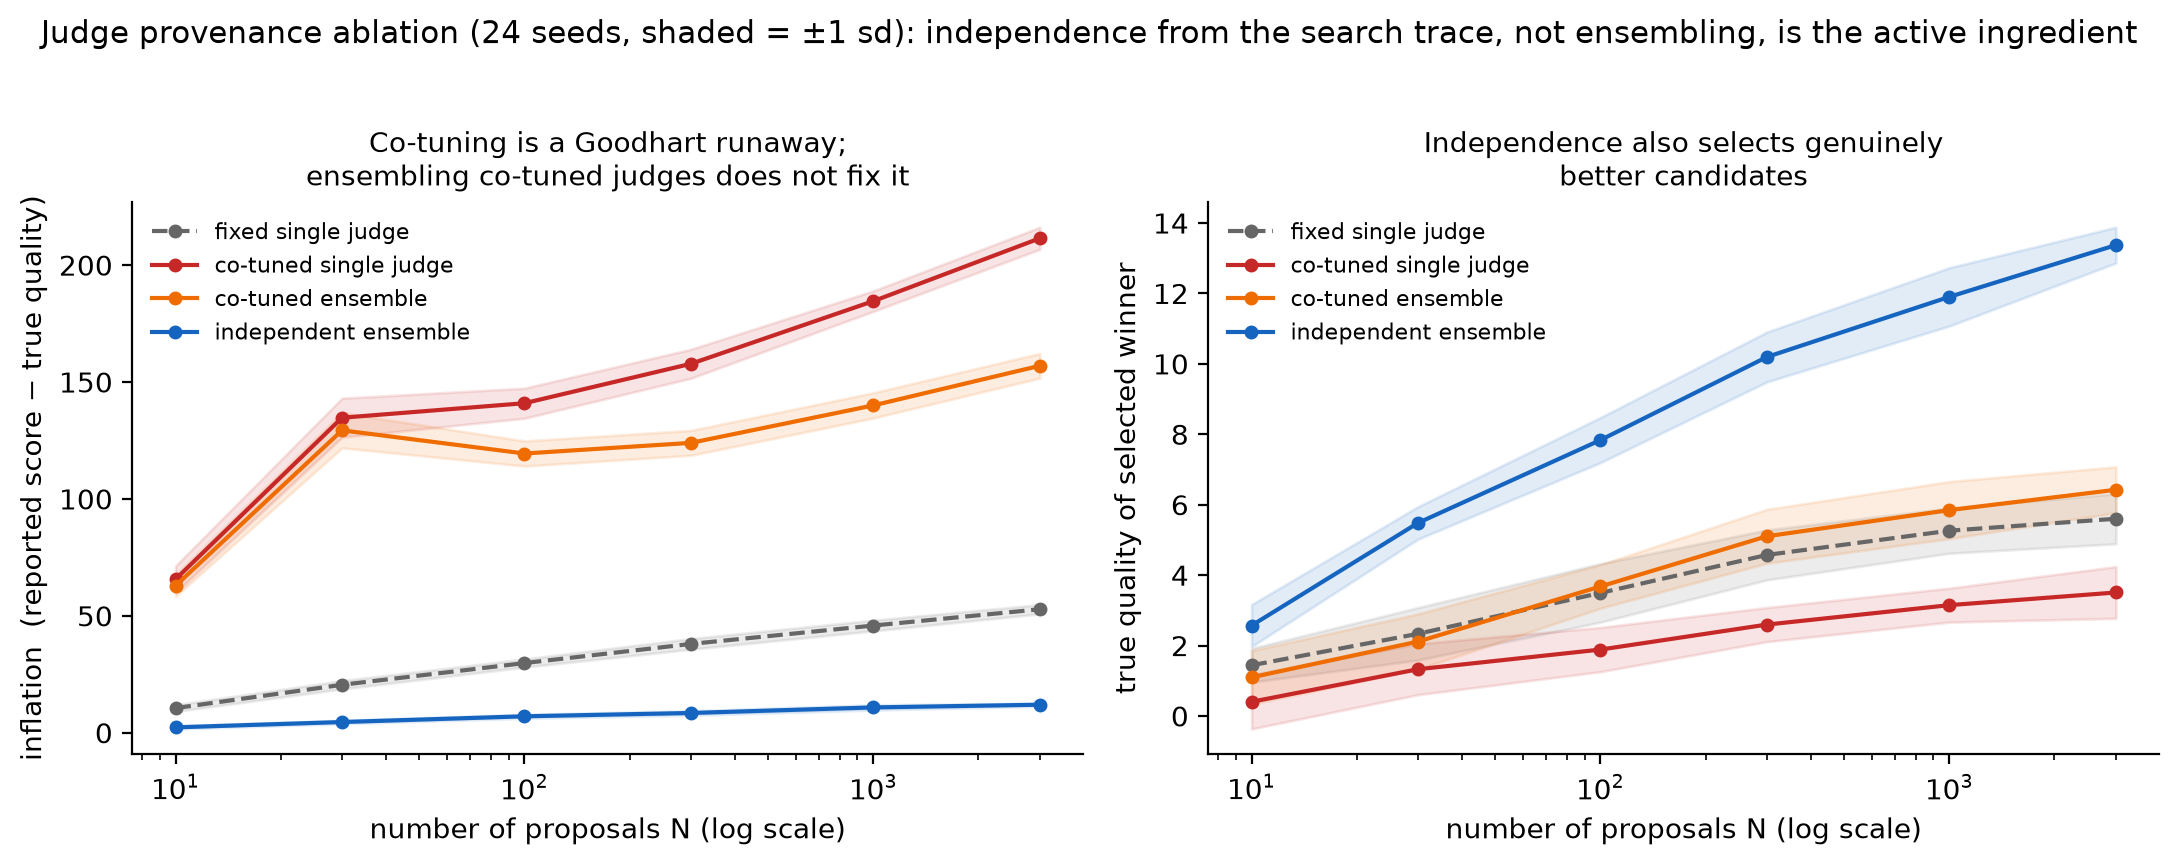
\includegraphics[width=\linewidth]{fig_ablation_cotuned.png}
\caption{Judge-provenance ablation across $N$ (24 seeds; bands $\pm1$~sd). Left: the calibration gap under co-tuning (B, C) dwarfs the static judge (A) and keeps growing; the trace-independent ensemble (D) stays nearly flat. Right: D also selects winners of far higher \emph{true} quality; the co-tuned judge (B) selects the worst.}
\label{fig:ablation}
\end{figure}

\textbf{Co-tuning is a Goodhart runaway (H1).} The co-tuned judge's gap is $211.5$ vs the static judge's $52.8$ at $N{=}3{,}000$ ($4.0\times$; the ratio is at least $4\times$ at every $N$ and as high as ${\sim}6.5\times$ at small $N$; directional pass rates recorded at $N{=}3{,}000$: 24/24 seeds) (Table~\ref{tab:ablation}, Fig.~\ref{fig:ablation}). The mechanism is mutual: the judge's quirk grows along the directions the generator concentrates in, the generator chases the enlarged quirk, and reported score compounds while true quality is left behind---indeed B's \emph{true} quality ($3.5$) is the worst of all conditions, below even the static-judge baseline ($5.6$). A co-tuned judge is not a noisier judge; it is an accomplice. Part of B's reported-score growth is the judge's own scale growing (the accumulated quirk norm compounds)---that is the runaway mechanism itself, not a confound, but it means B's inflation is measured in units that inflate with it. The scale-free confirmation is true quality: no rescaling of a judge can make its \emph{selections} genuinely worse, yet B selects the worst candidates of all four conditions.

\textbf{Ensembling without independence fails (H2).} The co-tuned ensemble retains a gap of $156.9$---$13.1\times$ the independent ensemble's $12.0$ at $N{=}3{,}000$, and the ratio is even larger at small $N$ (${\sim}27\times$). Averaging judges whose errors were correlated by the shared trace cancels almost nothing; this is the inference-time analogue of ensemble herding~\cite{eisenstein2023}, and it holds in 100\% of seeds.

\textbf{Independence is the active ingredient (H3, H4).} The trace-independent ensemble is the only condition whose reported score stays close to truth (gap $2.3\to12.0$ across the whole sweep), and it simultaneously selects the genuinely best candidates: true quality $13.4$ vs $5.6$ (static) and $3.5$ (co-tuned) at $N{=}3{,}000$. Independence pays twice---calibration and selection quality---and both margins hold in 24/24 seeds.

\section{Discussion}
For anyone building generate-and-select agents---strategy search, self-refining coders, automated red-teaming, prompt optimization---the operational rule is: \emph{a judge that was tuned, prompted, or patched using the pipeline's own outputs is part of the attack surface, not ground truth}. ``The judge said it was good'' is closer to in-sample fit than to evaluation. The measured fix is cheap: hold out judges that have never seen the generator's trace, and aggregate across them; ensembling alone, without that independence, recovers little. The same risk statement covers benchmark--system co-evolution (leaderboards patched in response to the systems they rank) and self-refinement loops whose critique signal is the generator's own~\cite{wang2022,pan2024}.

\textbf{Preliminary live instantiation.} A micro-scale live run (LLM generator and LLM judges, one-line predictor expressions over five features with objective held-out $R^2$ as ground truth; 2 seeds $\times$ 3 rounds, all completions cached) reproduces the core phenomenon with a real judge: the selecting judge rates its final winner $8.0/10$ while three held-out judges rate the same winner $5.3$ (self-inflation gap $+2.7$), and the winners' \emph{objective} quality is negative ($R^2<0$)---high reported scores on genuinely poor candidates. Selecting on the independent three-judge ensemble nearly closes the self-inflation gap ($+0.3$). At this scale the co-tuned and fixed single-judge conditions did not separate (identical trajectories); establishing the co-tuning amplification live requires a larger run and is the immediate next step. Script and cached completions: \texttt{llm\_judge\_instantiation.py}.

\section{Limitations and Next Step}
The testbed is synthetic and linear by design---provenance is the only manipulated variable, which is what makes the ablation clean, but effect \emph{sizes} here are not predictions for any real system. Co-tuning is one operationalization (taste refit toward round winners); prompt-iteration on real LLM judges may be gentler or harsher. The preliminary live run above confirms single-judge self-inflation and the independent-ensemble fix with a real LLM judge, but is far too small to test the co-tuning amplification; scaling that live run (more rounds, more seeds, richer domains) is the immediate next step. The mechanism is evaluator-agnostic and the prediction is unambiguous.

\section*{Reproducibility}
Deterministic, dependency-free, seeded: \texttt{ablation\_cotuned.py} (this ablation; 24 reseeds $\times$ 12 runs, directional pass rates emitted with the table) and \texttt{evaluator\_overfit\_demo.py} / \texttt{evaluator\_overfit\_robustness.py} (the static-judge baseline), each writing its results JSON alongside the script.

\bibliographystyle{ACM-Reference-Format}
\begin{thebibliography}{19}
\small
\bibitem{gao2023} L.~Gao, J.~Schulman, and J.~Hilton. 2023. Scaling Laws for Reward Model Overoptimization. \emph{Proc. ICML}, PMLR 202, 10835--10866.
\bibitem{coste2024} T.~Coste, U.~Anwar, R.~Kirk, and D.~Krueger. 2024. Reward Model Ensembles Help Mitigate Overoptimization. \emph{ICLR}. arXiv:2310.02743.
\bibitem{eisenstein2023} J.~Eisenstein et al. 2023. Helping or Herding? Reward Model Ensembles Mitigate but do not Eliminate Reward Hacking. arXiv:2312.09244.
\bibitem{itrh2025} H.~Khalaf, C.~Mayrink Verdun, A.~Oesterling, H.~Lakkaraju, and F.~du Pin Calmon. 2025. Inference-Time Reward Hacking in Large Language Models. \emph{NeurIPS}. arXiv:2506.19248.
\bibitem{pan2024} J.~Pan et al. 2024. Spontaneous Reward Hacking in Iterative Self-Refinement. arXiv:2407.04549.
\bibitem{prefleak2025} D.~Li et al. 2025. Preference Leakage: A Contamination Problem in LLM-as-a-Judge. arXiv:2502.01534.
\bibitem{zheng2023} L.~Zheng et al. 2023. Judging LLM-as-a-Judge with MT-Bench and Chatbot Arena. \emph{NeurIPS Datasets and Benchmarks}.
\bibitem{poll2024} P.~Verga et al. 2024. Replacing Judges with Juries: Evaluating LLM Generations with a Panel of Diverse Models. arXiv:2404.18796.
\bibitem{cheating2025} X.~Zheng, T.~Pang, C.~Du, Q.~Liu, J.~Jiang, and M.~Lin. 2025. Cheating Automatic LLM Benchmarks: Null Models Achieve High Win Rates. \emph{ICLR}. arXiv:2410.07137.
\bibitem{judgedeceiver2024} J.~Shi et al. 2024. Optimization-based Prompt Injection Attack to LLM-as-a-Judge. \emph{Proc. CCS}. arXiv:2403.17710.
\bibitem{bailey2014dsr} D.~H. Bailey and M.~L\'opez de Prado. 2014. The Deflated Sharpe Ratio. \emph{J. Portfolio Management} 40, 5, 94--107.
\bibitem{stw1999} R.~Sullivan, A.~Timmermann, and H.~White. 1999. Data-Snooping, Technical Trading Rule Performance, and the Bootstrap. \emph{J. Finance} 54, 5, 1647--1691.
\bibitem{flageat2025} M.~Flageat, J.~Huber, F.~H\'el\'enon, S.~Doncieux, and A.~Cully. 2025. Extract-QD Framework: Quality-Diversity in Noisy, Stochastic or Uncertain Domains. \emph{Proc. GECCO}.
\bibitem{wang2022} X.~Wang et al. 2022. Self-Consistency Improves Chain of Thought Reasoning in Language Models. arXiv:2203.11171.
\bibitem{goodhart1975} C.~A.~E. Goodhart. 1975. Problems of Monetary Management: The U.K. Experience. \emph{Papers in Monetary Economics}, Reserve Bank of Australia.
\end{thebibliography}

\end{document}
